\documentclass[12pt]{beamer}
\usetheme{Pittsburgh}
\usepackage[utf8]{inputenc}
\usepackage[english]{babel}
\usepackage{amsmath}
\usepackage{amsfonts}
\usepackage{amssymb}
\usepackage{graphicx}
\author{Sebastian Valet, Johannes Walter}
\title{Human Capital Investments and Expectations about Career and Family}
%\setbeamercovered{transparent} 
%\setbeamertemplate{navigation symbols}{} 
%\logo{} 
%\institute{} 
%\date{} 
%\subject{} 
\begin{document}

\begin{frame}
\titlepage
\end{frame}

%\begin{frame}
%\tableofcontents
%\end{frame}

% These two silde can probably go in the appendix
\begin{frame}{Current Population Characteristics I}
    \begin{itemize}
        \item Earnings, employment, and marriage data  for the US population using the 2009
        \item Not suited for causal inference; needs not reflect the student's beliefs
        \item Data from older cohort; includes not only high-ability participants
        \item But data is suited to document that career and family outcomes differ by educational choices in observational data
    \end{itemize}
\end{frame}

\begin{frame}{Current Population Characteristics II}
    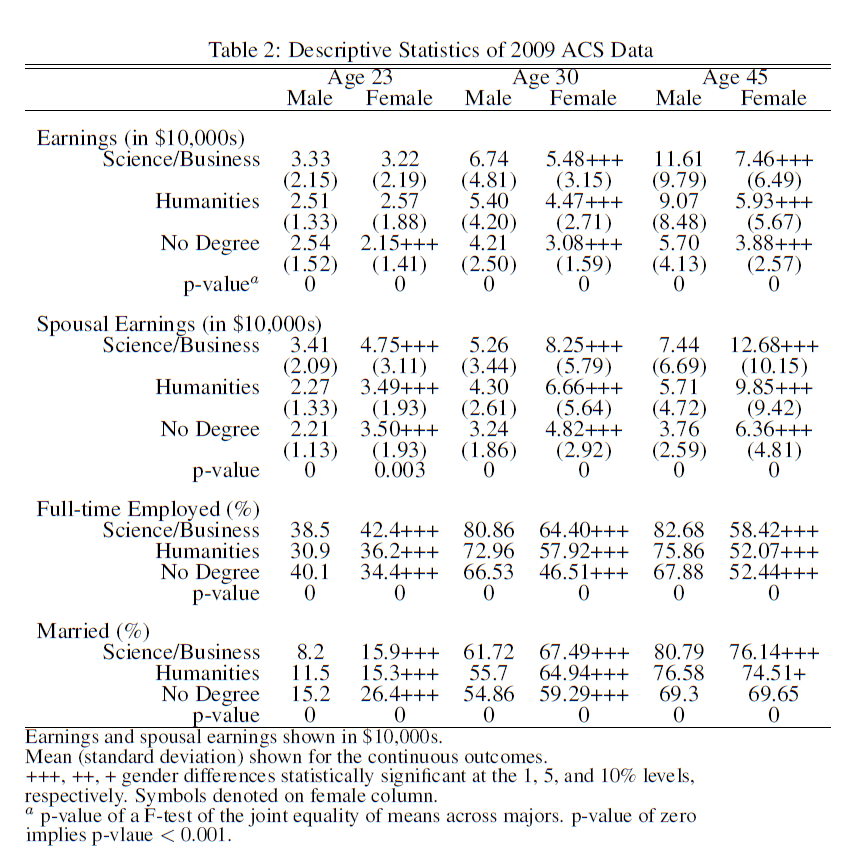
\includegraphics[scale=0.4]{Table2.png}
\end{frame}

\end{document}